\documentclass[tikz,border=2pt]{standalone}
\usepackage{amsmath,amssymb}
\usetikzlibrary{arrows.meta,decorations.pathreplacing}
\begin{document}
% One job with net service time S_0 = 3 (time units) and N = 2 failures. Bottom: the service clock,
% on which failures form a Poisson process of rate lambda_f (here at service times 1.2 and 1.8).
% Top: real time; each failure stops the job for a repair R_i, after which service resumes, so the
% effective service time is S = S_0 + R_1 + R_2.
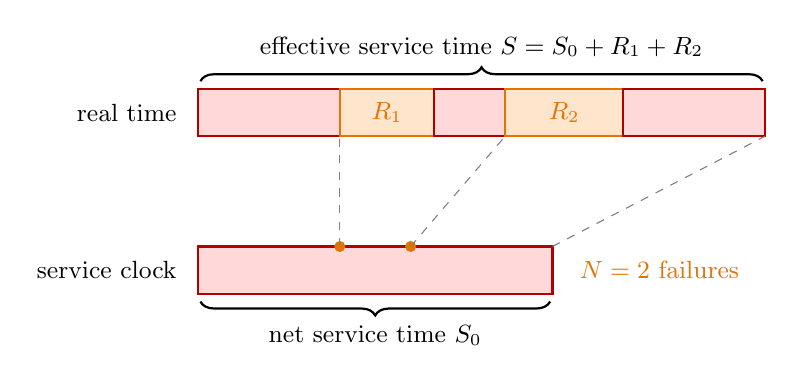
\begin{tikzpicture}[font=\small, >={Latex[length=2mm]}, x=1.5cm, y=1cm]
  \tikzset{job/.style={draw=red!70!black, fill=red!15, thick},
           outage/.style={draw=orange!90!black, fill=orange!20, thick}}
  % real time
  \node[anchor=east] at (-0.1,2.3) {real time};
  \draw[job] (0,2) rectangle (1.2,2.6);
  \draw[outage] (1.2,2) rectangle (2.0,2.6); \node[orange!90!black] at (1.6,2.3) {$R_1$};
  \draw[job] (2.0,2) rectangle (2.6,2.6);
  \draw[outage] (2.6,2) rectangle (3.6,2.6); \node[orange!90!black] at (3.1,2.3) {$R_2$};
  \draw[job] (3.6,2) rectangle (4.8,2.6);
  \draw[decorate, decoration={brace, amplitude=5pt}, thick] (0.02,2.7) -- (4.78,2.7)
    node[midway, above=5pt] {effective service time $S=S_0+R_1+R_2$};
  % service clock
  \node[anchor=east] at (-0.1,0.3) {service clock};
  \draw[job] (0,0) rectangle (3,0.6);
  \foreach \t in {1.2,1.8} \fill[orange!90!black] (\t,0.6) circle (2pt);
  \draw[decorate, decoration={brace, amplitude=5pt, mirror}, thick] (0.02,-0.1) -- (2.98,-0.1)
    node[midway, below=5pt] {net service time $S_0$};
  \node[orange!90!black, anchor=west] at (3.15,0.3) {$N=2$ failures};
  % link failure epochs
  \draw[gray, dashed] (1.2,0.6) -- (1.2,2);
  \draw[gray, dashed] (1.8,0.6) -- (2.6,2);
  \draw[gray, dashed] (3,0.6) -- (4.8,2);
\end{tikzpicture}
\end{document}
